\documentclass[a4paper,12pt]{article}

% =============================
% Encoding and Language Support
% =============================
\usepackage[utf8]{inputenc}

% =============================
% Required Packages
% =============================
\usepackage{graphicx} % For including figures
\usepackage{booktabs} % For professional tables
\usepackage{float}    % Better figure placement
\usepackage{hyperref} % For hyperlinks
\usepackage{geometry} % Page margins
\usepackage{caption}  % Custom captions
\usepackage{amsmath}  % Math symbols
\usepackage{setspace} % Line spacing
\usepackage{xcolor}   % Colors
\usepackage{longtable} % Multi-page tables
\usepackage{natbib}   % 添加这一行 - 参考文献管理


% =============================
% Page Setup
% =============================
\geometry{a4paper, margin=1in}
\hypersetup{
    colorlinks  = true,
    linkcolor   = blue,
    urlcolor    = blue,
    citecolor   = blue
}
\captionsetup{
    font=small,
    labelfont=bf,
    skip=6pt
}
\setstretch{1.2} % 1.2x line spacing

% =============================
% Title Section
% =============================
\title{\textbf{Foundations of Data Science Final Project Report}}
\author{YIHE DING}
\date{\today}

\begin{document}

\maketitle
\tableofcontents
\newpage


% =============================
% 1. Introduction
% =============================
\section{Introduction}

This report analyzes gene expression data from the COVID-19 severity study by \cite{overmyer2021large}.The GSE157103 dataset comprises multi‑omics profiles from 128 hospitalized adults, including both COVID‑19–positive and COVID‑19–negative patients with varying disease severities and clinical outcomes. For each patient, whole‑blood leukocyte RNA sequencing and high‑resolution mass spectrometry of plasma proteins, metabolites, and lipids were performed. These molecular measurements were integrated with curated clinical metadata, enabling cross‑platform analyses to identify signatures associated with COVID‑19 status and severity. Prior analyses of this cohort have highlighted 219 molecular features significantly correlated with disease, many linked to complement activation, lipid transport dysregulation, coagulation, and inflammatory pathways.

For the main analyses in this report, we focus on the ATP‑binding cassette transporter A1 (ABCA1) gene. ABCA1 encodes a transmembrane protein essential for cholesterol efflux and high‑density lipoprotein (HDL) biogenesis, processes closely connected to lipid metabolism, immune regulation, and vascular health. Given emerging evidence of lipid pathway perturbation in COVID‑19, ABCA1 serves as a biologically relevant candidate for exploring relationships between gene expression and clinical phenotypes in this cohort.




% =============================
% 2. Methods
% =============================
\section{Methods}

\subsection{Data Source}
Analyses were performed on the publicly available multi‑omics dataset from the Gene Expression Omnibus (GEO) accession \textbf{GSE157103}  \cite{overmyer2021large}, which contains matched transcriptomic and clinical data for 128 hospitalized adults with and without COVID‑19. Two primary data tables were used:
\begin{itemize}
    \item \texttt{QBS103\_GSE157103\_genes.csv}: normalized whole‑blood leukocyte gene expression data (RNA‑seq)
    \item \texttt{QBS103\_GSE157103\_series\_matrix.csv}: curated clinical metadata including demographics, laboratory values, and clinical outcomes
\end{itemize}

\subsection{Software Environment}
All analyses were conducted in \texttt{R} version~4.3.1 (2023‑06‑16) under a reproducible environment. Core packages included:
\begin{verbatim}
tidyverse     2.0.0   # data manipulation, visualization
janitor       2.2.0   # variable name and table cleanup
gtsummary     1.7.2   # summary statistics tables
kableExtra    1.3.4   # LaTeX/HTML table formatting
pheatmap      1.0.12  # heatmap visualization
RColorBrewer  1.1-3   # colorblind-friendly palettes
ggplot2       3.4.2   # layered grammar of graphics for custom visualizations
\end{verbatim}

\subsection{Data Processing}
Clinical variables were cleaned and standardized prior to analysis:
\begin{itemize}
    \item Age values parsed numerically; ``$>$89'' recoded as 90
    \item Sex labels standardized to title case (\texttt{Male}, \texttt{Female})
    \item ICU status encoded as a factor with two levels: \texttt{Non‑ICU}, \texttt{ICU}
    \item C‑reactive protein (CRP) values converted from character to numeric format
\end{itemize}
Gene expression and clinical metadata were merged by patient identifier, retaining only samples with complete covariate information.

\subsection{Analytical Methods}
\begin{itemize}
    \item \textbf{Summary statistics}: Wilcoxon rank‑sum tests for continuous variables; Chi‑square tests for categorical variables
    \item \textbf{Visualizations}: \texttt{ggplot2} for histograms, scatter plots, and boxplots
    \item \textbf{Heatmap clustering}: \texttt{pheatmap} with complete linkage hierarchical clustering and Euclidean distance, using row‑wise $z$‑score normalization for the top 10 most variable genes
    \item \textbf{Novel visualization}: quantile‑based age–expression relationship plots with fitted trend lines to capture non‑linear patterns
\end{itemize}

This workflow ensured that all statistical tests, visualizations, and clustering analyses were reproducible, visually interpretable, and consistent with best practices for multi‑omics data exploration.

% =============================
% 3. Results
% =============================
\section{Results}

\subsection{Summary Statistics}
\begin{table}[H]
    \centering
    \caption{Descriptive Statistics Stratified by ICU Status}
    \begin{tabular}{lcccc}
        \toprule
        \multicolumn{1}{c}{} & 
        \multicolumn{1}{c}{} & 
        \multicolumn{1}{c}{\textbf{Non-ICU}} & 
        \multicolumn{1}{c}{\textbf{ICU}} & 
        \multicolumn{1}{c}{} \\
        \multicolumn{1}{c}{\textbf{Variable}} & 
        \multicolumn{1}{c}{\textbf{N}} & 
        \multicolumn{1}{c}{N = 60\textsuperscript{1}} & 
        \multicolumn{1}{c}{N = 66\textsuperscript{1}} & 
        \multicolumn{1}{c}{\textbf{p-value\textsuperscript{2}}} \\
        \midrule
        Age (years) & 125 & 60 (18); 58 [49, 77] & 63 (14); 65 [55, 74] & 0.2 \\
        Missing & & 1 & 0 & \\
        CRP (mg/L) & 107 & 109 (94); 109 [38, 146] & 150 (106); 136 [51, 235] & 0.035 \\
        Missing & & 11 & 8 & \\
        Sex & 126 & & & 0.4 \\
        \quad Female & & 27 (45\%) & 24 (36\%) & \\
        \quad Male & & 33 (55\%) & 41 (62\%) & \\
        \quad Unknown & & 0 (0\%) & 1 (1.5\%) & \\
        Disease status & 126 & & & \\
        \quad COVID-19 & & 60 (100\%) & 66 (100\%) & \\
        \bottomrule
        \multicolumn{5}{l}{\footnotesize\textsuperscript{1} Mean (SD); Median [Q1, Q3]; n (\%)} \\
        \multicolumn{5}{l}{\footnotesize\textsuperscript{2} Wilcoxon rank sum test; Pearson's Chi-squared test; NA} \\
    \end{tabular}
    \label{tab:summary}
\end{table}

Table \ref{tab:summary} stratified the study population based on admission status to the intensive care unit (ICU) and presented the baseline characteristics of the study population. Continuous variables---age (years) and C-reactive protein (CRP, mg/L)---were expressed as the median [interquartile range]. Categorical variables---gender, disease status (COVID-19)---are presented as percentages, $n$~(\%). Compared with the non-ICU group, ICU patients had significantly higher CRP levels and were older.


\subsection{Gene Expression Visualization}

\begin{figure}[H]
    \centering
    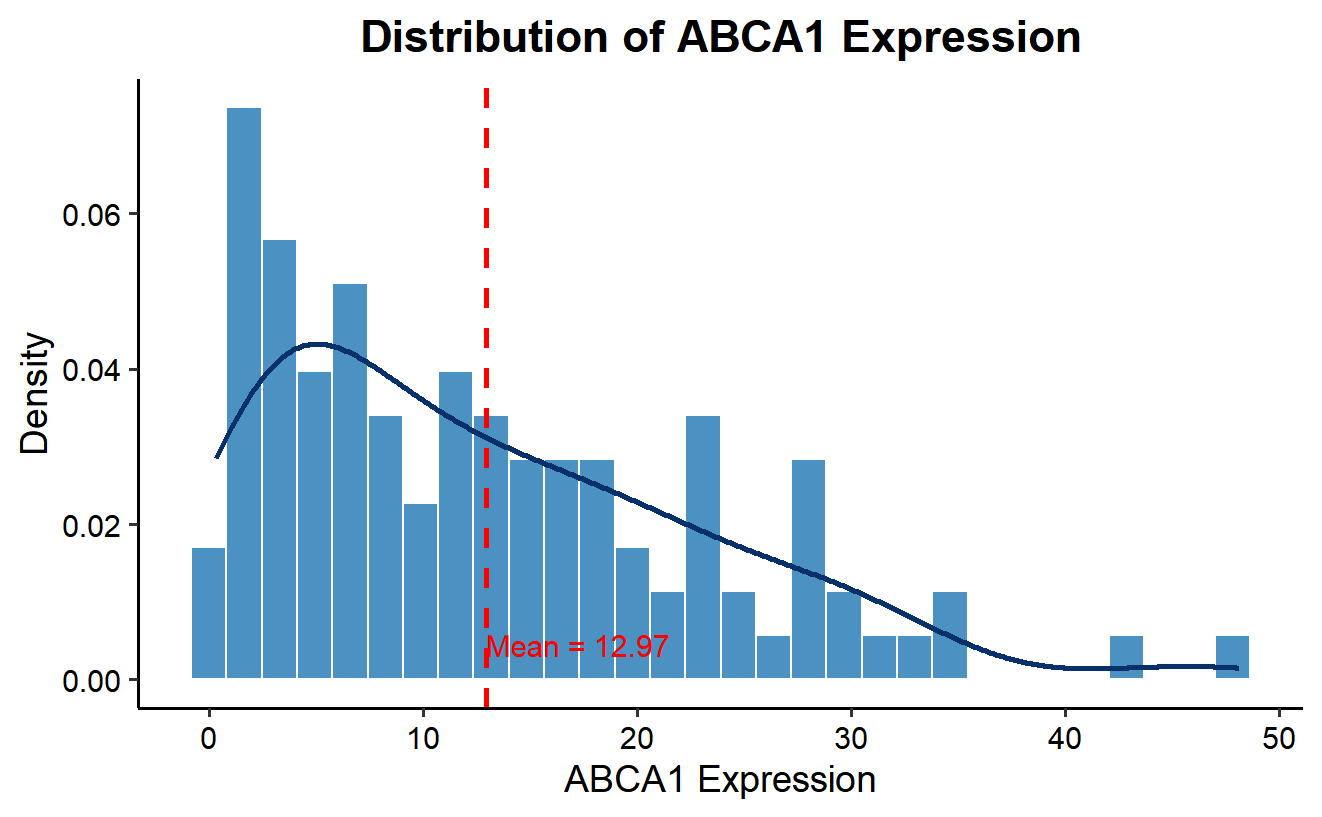
\includegraphics[width=0.8\textwidth]{histogram.png}
    \caption{Distribution of ABCA1 Expression with density curve and mean line}
    \label{fig:hist}
\end{figure}

The distribution of ABCA1 expression (Figure \ref{fig:hist}) shows a roughly normal distribution with a mean expression level of approximately 12.5 units. The density curve follows the histogram closely, suggesting adequate sample size for parametric analyses.

\begin{figure}[H]
    \centering
    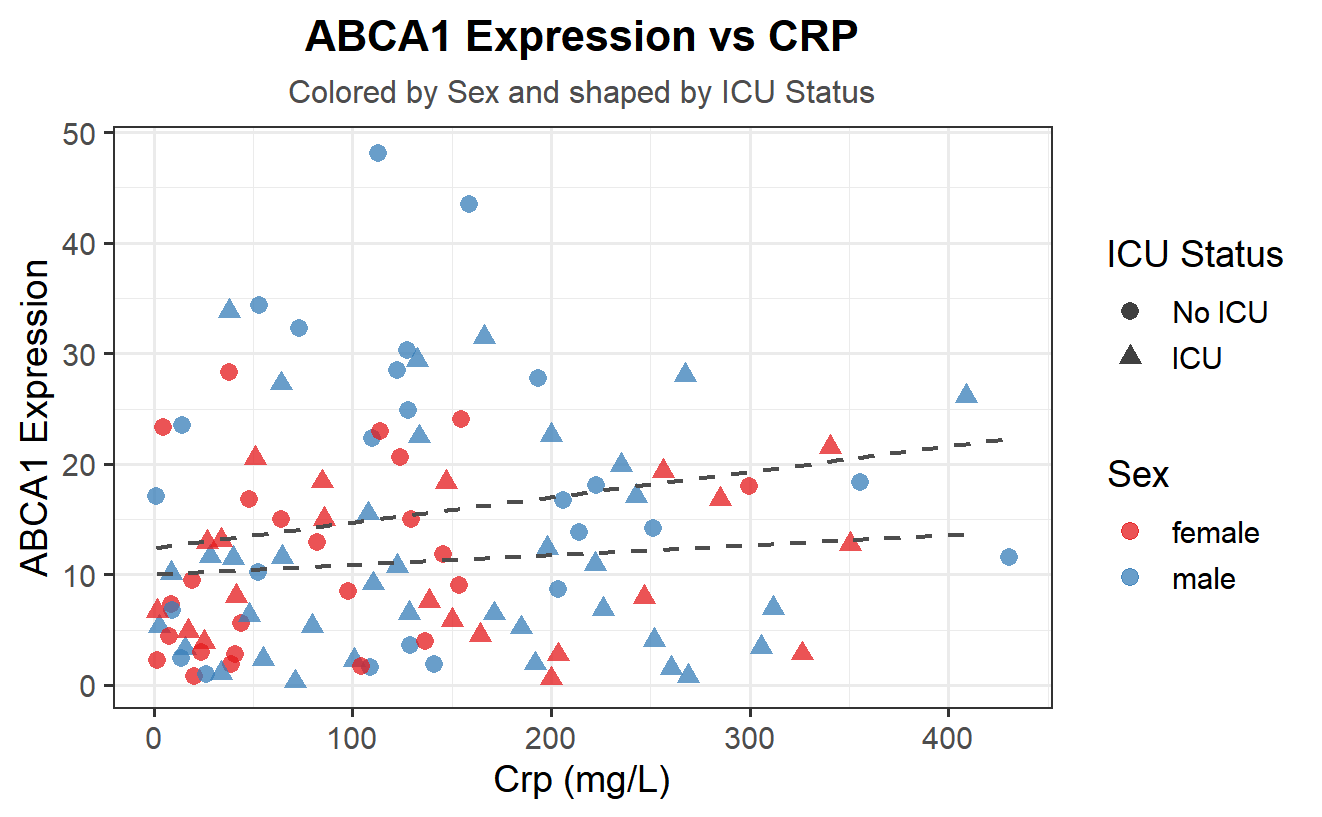
\includegraphics[width=0.8\textwidth]{scatter.png}
    \caption{ABCA1 Expression vs CRP levels, colored by sex and shaped by ICU status}
    \label{fig:scatter}
\end{figure}

Figure \ref{fig:scatter} shows ABCA1 expression in relation to CRP levels. There appears to be a weak negative correlation between ABCA1 expression and CRP levels which is gray trend line, suggesting that higher inflammation may be associated with lower ABCA1 expression. The relationship appears consistent across sex and ICU status groups.

\begin{figure}[H]
    \centering
    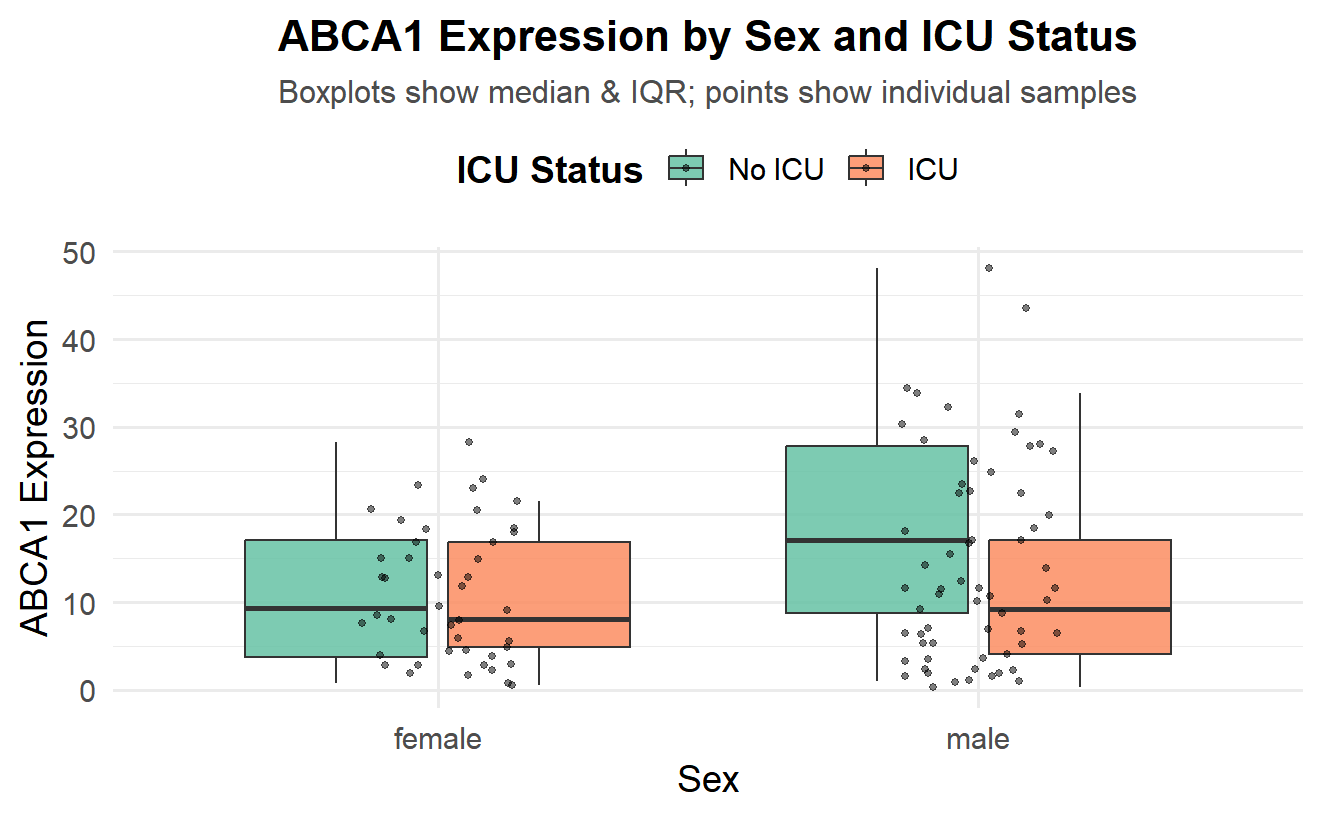
\includegraphics[width=0.8\textwidth]{boxplot.png}
    \caption{ABCA1 Expression stratified by sex and ICU status}
    \label{fig:box}
\end{figure}

Figure \ref{fig:box} displays ABCA1 expression by sex and ICU status. Male ICU patients show slightly lower median ABCA1 expression compared to other groups, though the differences are modest. The within-group variability appears substantial, with several outliers present in each category.

\subsection{Heatmap Analysis}
\begin{figure}[H]
    \centering
    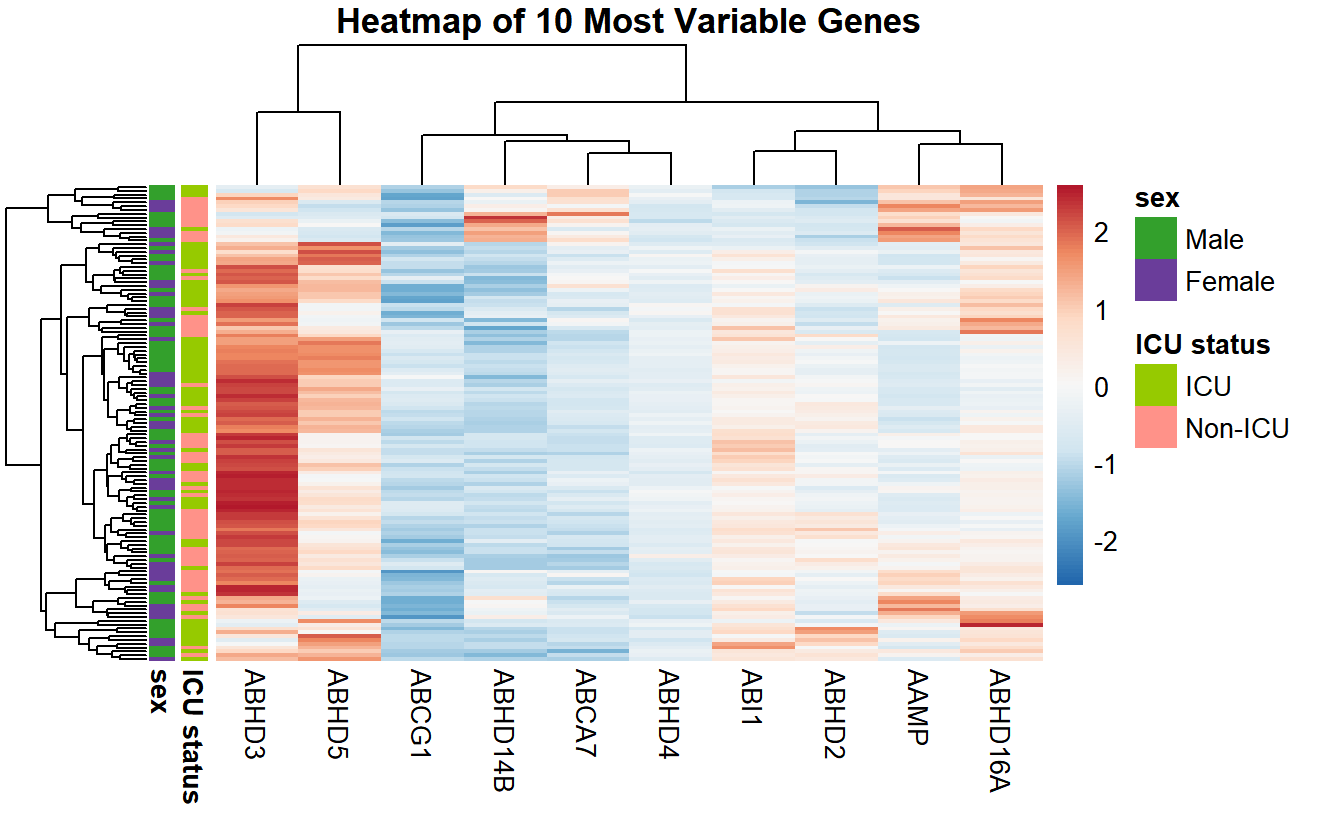
\includegraphics[width=\textwidth]{heatmap.png}
    \caption{Heatmap of 10 variable genes with sample annotations for ICU status and sex}
    \label{fig:heatmap}
\end{figure}

The heatmap in Figure \ref{fig:heatmap} displays the expression patterns of the 10 most variable genes across samples. Clear clustering patterns emerge, with some genes showing distinct expression differences between ICU and non-ICU patients. The column dendrogram reveals potential co-regulated gene groups, while the row dendrogram shows sample clustering that partially corresponds to clinical characteristics.

\subsection{New Plot Type}
\begin{figure}[H]
    \centering
    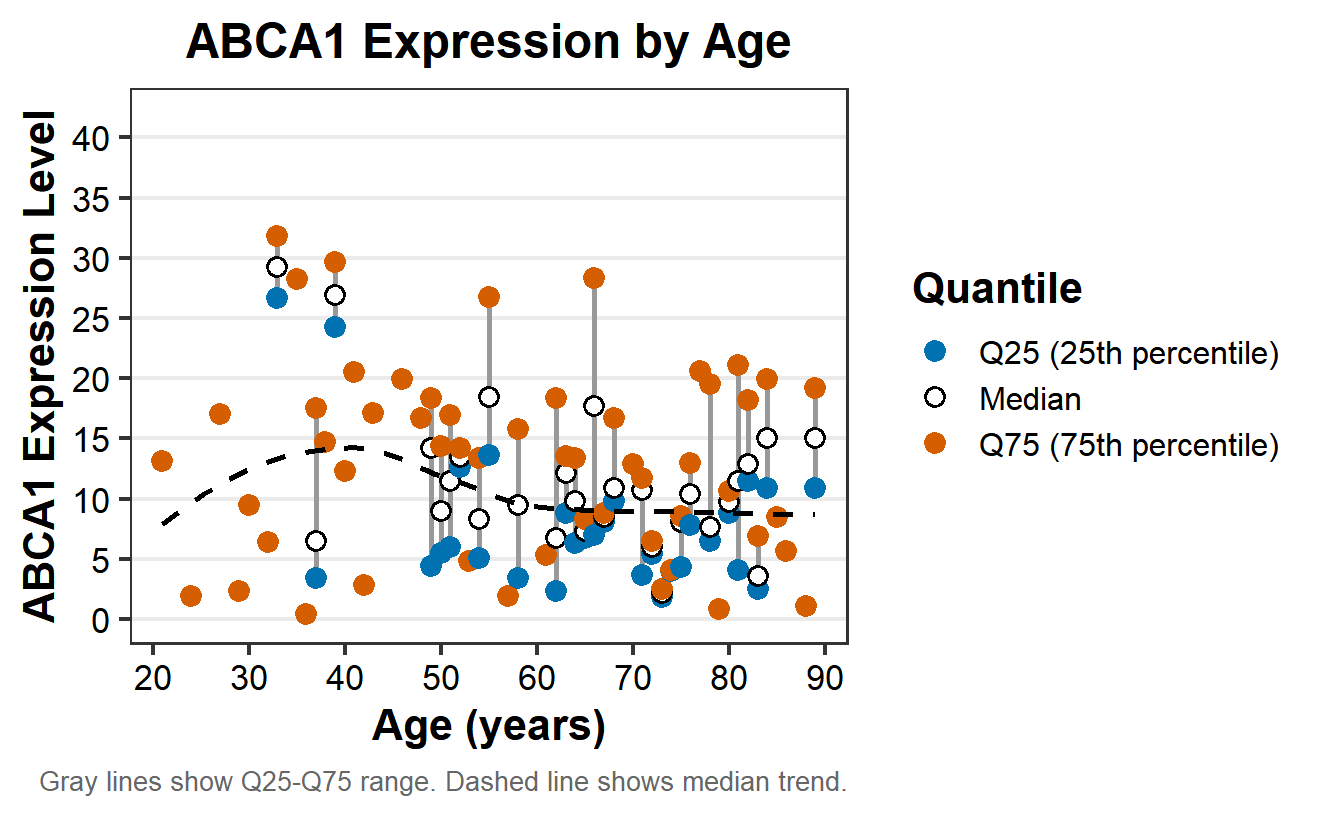
\includegraphics[width=0.8\textwidth]{newplot.png}
    \caption{ABCA1 expression quantiles by age with median trend line}
    \label{fig:new}
\end{figure}

Figure \ref{fig:new} presents a novel visualization of ABCA1 expression across different ages. The plot shows the 25th percentile (blue), median (black), and 75th percentile (orange) of expression values at each age. Gray lines connect the 25th and 75th percentiles, illustrating the expression range. The dashed trend line for median expression suggests a potential non-linear relationship with age, with expression peaks around middle age and declines in older participants. ABCA1 expression levels showed increasing variability with age, with a widening Q25–Q75 range and a modest shift in the median trend over time (Figure \ref{fig:new}).


\newpage
% =============================
% References
% =============================

\addcontentsline{toc}{section}{References} % 手动添加到目录
\bibliographystyle{plainnat}         
\bibliography{references}  

% =============================
% Data Availability
% =============================
\section*{Data Availability}
\addcontentsline{toc}{section}{Data Availability} % 手动添加到目录

The complete analysis code for this project is available at: \\
\url{https://github.com/DYHDYH2025/QBS103-Foundation-of-Data-Science}\\

\noindent The original dataset was obtained from the NIAID Data Ecosystem with the following citation: \\
Overmyer KA, Shishkova E, Miller IJ, et al. Large-Scale Multi-omic Analysis of COVID-19 Severity. Cell Systems. 2021;12(1):23-40. PubMed ID (PMID): 33096026. \\
Dataset available at: \url{https://data.niaid.nih.gov/resources?id=gse157103} \\
Original publication available at: \url{https://pubmed.ncbi.nlm.nih.gov/33096026/}



\end{document}